\documentclass{article}
\usepackage[utf8]{inputenc}
\usepackage{multicol}
\usepackage{listings}
\usepackage{verbatim}
\usepackage{color}
\usepackage{geometry}
\usepackage{float}
\floatstyle{boxed}
\restylefloat{figure}
\usepackage{amsmath}
\usepackage[svgnames]{xcolor}
\definecolor{ocre}{RGB}{243,102,25}
\usepackage{caption}
\usepackage[font={color=black},figurename=Fig.,labelfont={it}]{caption}
%\captionsetup{labelformat=empty,color=red}
\usepackage{pdflscape}
\usepackage{hyperref}
\setlength{\belowcaptionskip}{-10pt}
\setlength{\abovecaptionskip}{-30pt}

\usepackage{graphicx}
\definecolor{codegreen}{rgb}{0,0.6,0}
\definecolor{codegray}{rgb}{0.5,0.5,0.5}
\definecolor{codepurple}{rgb}{0.58,0,0.82}
\definecolor{backcolour}{rgb}{0.95,0.95,0.92}

\lstdefinestyle{mystyle}{
	backgroundcolor=\color{backcolour},   
	commentstyle=\color{codegreen},
	keywordstyle=\color{blue},
	numberstyle=\tiny\color{codegray},
	stringstyle=\color{codepurple},
	basicstyle=\footnotesize,
	breakatwhitespace=false,         
	breaklines=true,                 
	captionpos=b,                    
	keepspaces=true,                 
	numbers=left,                    
	numbersep=5pt,                  
	showspaces=false,                
	showstringspaces=false,
	showtabs=false,                  
	tabsize=2
}

\lstset{style=mystyle}
\title{Image Processing\\
	Home work 06\\Color Spaces  }
\author{Aqeel Labash\\ \textbf{Lecturer:} Gholamreza Anbarjafari}
\date{19 April 2016}

\geometry{
	a4paper,
	total={170mm,257mm},
	left=10mm,
	top=5mm,
}
\begin{document}
	\maketitle
	\begin{multicols*}{2}
	\section*{CIE 1931 XYZ}
	It's the first quantitative that links the pure physical colors with electromagnetic visible spectrum.\cite{2} This color space allow physical radiation responses to color inks, illuminated displays, recording devices.\cite{2} This model try to imitate the eye cones (LMS-Long,Middle,Short) using XYZ.\cite{2}
	\subsection*{CIELUV}
	CIELUV is simple to compute transformation from the previous one. It's used in computer graphics which deal with colored light.
	\subsection*{CIELAB}
	This color space use L for lightness and \(a,b\) for color opponent dimensions. This color space is based on non-linearly compressed coordinates. \cite{3}
	\subsection*{CIEUVW}
	This color space is based on \href{https://en.wikipedia.org/wiki/CIE_1960_color_space}{CIE 1960 color space}.This color space was invented to have the ability to calculate the color differences without holding luminance as constant.
	\[ U^*=13W^*(u-u_0)\]
	\[ V^*=13W^*(v-v_0)\]
	\[ W^*=25Y^{\frac{1}{3}}-17\]
	Where \((u_0,v_0)\)represent the white point and \(Y\) represent the luminous \href{https://en.wikipedia.org/wiki/CIE_1931_color_space#Tristimulus_values}{tristimulus value}.\cite{4}
	\section*{RGB}
	In this color space each pixel is represented by 3 values R:Red, G:green , B:blue. RGB color space is any additive color space based on RGB.RGB is considered as good color model for computer graphics because human visual system works in similar but not identical way.\cite{5}
	\subsection*{sRGB}
	sRGB is in RGB color space, desinged by Hewlett-Packard and Microsoft to be used for monitors, printers and Internet.\cite{6}
	\subsection*{Adobe RGB}
	It's an RGB color space developed by Adobe in 1998. It was designed to get the ability to have colors achievable by CMYK color printers.Which means being able to have RGB that represent CMYK for screens.But in the end it encompass about 50\% of specified visible colors by CIELAB (Which is more than sRGB) \cite{7}
	\subsection*{Adobe Wide Gamut RGB}
	The wide-gamut RGB color space (or Adobe Wide Gamut RGB)is a RGB color space created by Adobe Systems. This color space provide large gamut(\textbf{Gamut} represent the subset of colors that the color space can represent\cite{9}).This color space has wider range than sRGB or Adobe RGB.It encompasses 77.6 \% of CIELAB while Adobe RGB 52.1\% and sRGB 35.9\% \cite{8}
	\subsection*{Other RGB spaces}
	For RGB spaces it's open ended.Because picking new red,green,blue primaries and gamma value a new space could be invented.like \href{https://en.wikipedia.org/wiki/ProPhoto_RGB_color_space}{ProPhoto RGB color space} and \href{https://en.wikipedia.org/wiki/Rec._2020}{Rec. 2020}\cite{1}
	\section*{Luma plus chroma/chrominance}
	\subsection*{YIQ}
	YIQ color space is was used in some countries for NTSC TV colors.Y component represent the luma (brightness\cite{10}) \textbf{I} represent the in-phase, \textbf{Q} represent quadrature, referring to the components used in quadrature amplitude modulation.\cite{11}
	\begin{figure}[H]
	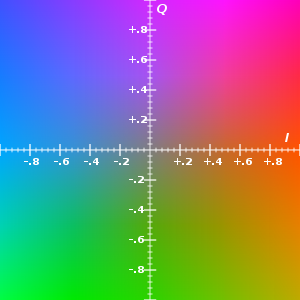
\includegraphics[scale=0.5]{YIQ.png}
	\caption{Colors at Y=0.5}
	\end{figure}
Example image showing YIQ components
\begin{figure}[H]
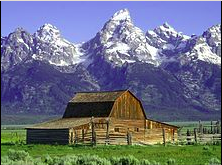
\includegraphics[scale=0.5]{YIQALL.png}
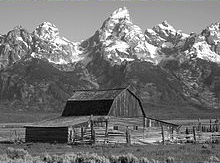
\includegraphics[scale=0.5]{Y.png}
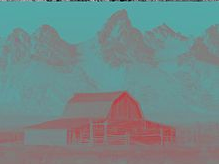
\includegraphics[scale=0.5]{I.png}

\includegraphics[scale=0.5]{Q.png}
\caption{Show YIQ components}
\end{figure}
\subsection*{Y'UV}
This color space defined in terms \(Y'\) for luma or brightness and \(UV\) for chrominance components.This color space used for PAL and SECAM video standards."Previous black-and-white systems used only luma (Y') information. Color information (U and V) was added separately via a sub-carrier so that a black-and-white receiver would still be able to receive and display a color picture transmission in the receiver's native black-and-white format".\cite{12}
\begin{figure}[H]
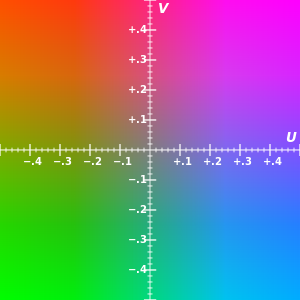
\includegraphics[scale=0.5]{YUV.png}
\caption{Colors in Y'UV when Y'=0.5}
\end{figure}
\begin{figure}[H]
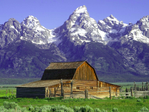
\includegraphics[height=35mm,width=35mm]{YUVall.png}
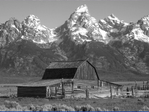
\includegraphics[height=35mm,width=35mm]{Yla.png}
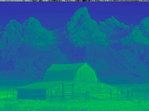
\includegraphics[height=35mm,width=35mm]{U.png}
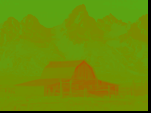
\includegraphics[height=35mm,width=35mm]{V.png}
\caption{Show Y'UV components}
\end{figure}
	\section*{CMYK}
	CMYK color model used for printing mainly where CMYK refere to C:Cyan , M:Magenta, Y:yellow,K:Key(black).This type actually descripe the printing process it self where the image is disassembled to these colors so the printer print the image. (Usually inkjet printers have those colors).And the printer also print the colors in the same order of the abbreviation.\cite{13}
	\begin{figure}[H]

\includegraphics[scale=0.7]{CMYK.png}
\caption{The CMYK colors}
	\end{figure}
	\begin{figure}[H]
	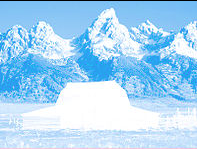
\includegraphics[height=35mm,width=35mm]{C.png}
	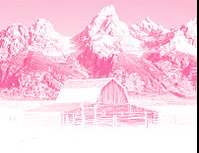
\includegraphics[height=35mm,width=35mm]{M.png}
	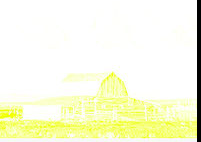
\includegraphics[height=35mm,width=35mm]{Yk.png}
	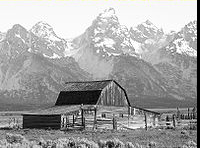
\includegraphics[height=35mm,width=35mm]{k.png}
	\caption{Show CMYK Components For the same image represented earlier}
	\end{figure}
	\textbf{Note:}Only the references in the third page due to lack of space.
	\begin{thebibliography}{9}
		\bibitem{1}
		\href{https://en.wikipedia.org/wiki/List_of_color_spaces_and_their_uses}{Color spaces and there uses}
		\bibitem{2}
		\href{https://en.wikipedia.org/wiki/CIE_1931_color_space}{CIE 1931}
		\bibitem{3}
		\href{https://en.wikipedia.org/wiki/Lab_color_space}{Label Color Space}
		\bibitem{4}
		\href{https://en.wikipedia.org/wiki/CIE_1964_color_space}{CIE 1964 color space}
		\bibitem{5}
		\href{https://en.wikipedia.org/wiki/RGB_color_space}{RGB color space}
		\bibitem{6}
		\href{https://en.wikipedia.org/wiki/SRGB}{sRGB}
		\bibitem{7}
		\href{https://en.wikipedia.org/wiki/Adobe_RGB_color_space}{Adobe RGB color space}
		\bibitem{8}
		\href{https://en.wikipedia.org/wiki/Wide-gamut_RGB_color_space}{Wide gamut RGB}
		\bibitem{9}
		\href{https://en.wikipedia.org/wiki/Gamut}{Gamut}
		\bibitem{10}
		\href{https://en.wikipedia.org/wiki/Luma_(video)}{Luma}
		\bibitem{11}
		\href{https://en.wikipedia.org/wiki/YIQ}{YIQ}
		\bibitem{12}
		\href{https://en.wikipedia.org/wiki/YUV}{YUV}
		\bibitem{13}
		\href{https://en.wikipedia.org/wiki/CMYK_color_model}{CMYK color model}
	\end{thebibliography}
	\end{multicols*}
\end{document}